\chapter{Introduction}\label{cp:introduction}

Ansys is a finite element solver used to computationally analyze structures. In this lab, Ansys was used to perform a structural analysis on a simply-supported truss, shown for reference in \autoref{fig:truss} with material properties given in \autoref{tab:truss}. The objective was to find the displacement at each node; the reaction forces at nodes \numlist{1;3}; and the forces, stresses, and volume in each member.

\begin{figure}[htpb]
    \centering
    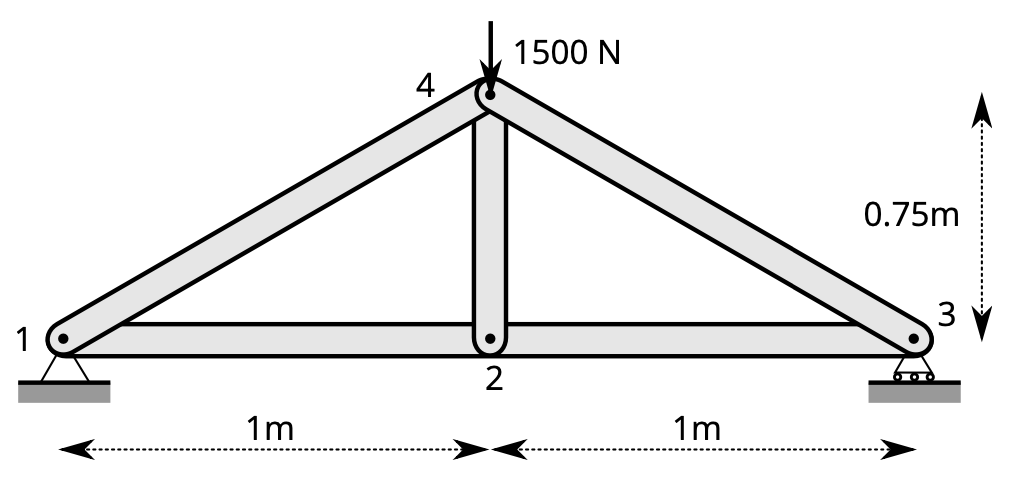
\includegraphics[width=\linewidth]{Figures/given_figure.png}
    \caption[Truss given in the lab manual]{Truss given in the lab manual \citep{runnels2024}.}
    \label{fig:truss}
\end{figure}

\begin{table}[htpb]
    \centering
    \caption[Given material properties]{The cross-sectional area \gls{A} and Young's modulus \gls{E} for each member in \autoref{fig:truss} \citep{runnels2024}.}
    \begin{tabular}{ccc}
    \toprule
    Member & \gls{E} $\left[\unit{\giga\pascal}\right]$ & \gls{A} $\left[\unit{\meter^2}\right]$ \\
    \midrule
    \numrange[range-phrase = --]{1}{2} & \num{210} & \num{0.00025} \\
    \numrange[range-phrase = --]{2}{3} & \num{210} & \num{0.00025} \\
    \numrange[range-phrase = --]{1}{4} & \num{70} & \num{0.00005} \\
    \numrange[range-phrase = --]{2}{4} & \num{70} & \num{0.00005} \\
    \numrange[range-phrase = --]{3}{4} & \num{70} & \num{0.00005} \\
    \bottomrule
\end{tabular}
    \label{tab:truss}
\end{table}